\documentclass[../../main.tex]{subfiles}
\graphicspath{{\subfix{../../image/}}} % 指定图片目录,后续可以直接使用图片文件名。

% 例如:
% \begin{figure}[H]
% \centering
% \includegraphics[scale=0.4]{image-01.01}
% \caption{图片标题}
% \label{figure:image-01.01}
% \end{figure}
% 注意:上述\label{}一定要放在\caption{}之后,否则引用图片序号会只会显示??.

\begin{document}

\section{映射与集合的基数}

\subsection{映射}

\begin{definition}[映射]
设 $A, B$ 为非空集, 若存在对应法则 $f$, 使得对每个 $x \in A$ 都有唯一确定的 $y \in B$ 与之对应, 则称对应法则 $f$ 为从 $A$ 到 $B$ 的映射. 记为 $f : A \to B$, 其表达形式为 $y = f(x), x \in A$.

$A$ 称为 $f$ 的\textbf{定义域}, 记为 $D(f)$.$B$称为$f$的\textbf{陪域}.
$A$ 在 $f$ 下的象称为 $f$ 的\textbf{值域}, 记为 $R(f)$, 即
\begin{align*}
R(f) = f(A) = \{f(x) : x \in A\}
\end{align*}

集合 $B_0 \subset B$ 在 $f$ 下的\textbf{原象}, 记为 $f^{-1}(B_0)$, 即
\begin{align*}
f^{-1}(B_0) = \{x \in A : f(x) \in B_0\}
\end{align*}
\end{definition}
\begin{remark}
关于映射的定义, 我们作以下几点说明:

(1) 对每一个 $x \in A$, 只能有唯一的 $y \in B$ 与它对应;并且$f$的一个像可以存在多个原像.

(2) $f(A) \subset B$, 不一定有 $f(A) = B$;

(3) 映射是由定义域和对应法则共同确定的, 但对应法则的表达形式可能不唯一. 例如
\begin{align*}
y = |x|, x \in \mathbb{R} \quad \text{ 和 } \quad y = \sqrt{x^2}, x \in \mathbb{R}
\end{align*}

(4) 值域中的元可以是集合. 例如 $A = \mathbb{N}, B = \{B_n\}_{n = 1}^{\infty}, \phi(n) = B_n$;

(5) 定义域中的元也可以是集合. 例如 $A$ 可列, $\mathcal{D} \subset 2^A$, 定义 $\phi : \mathcal{D} \to \{0\} \cup \mathbb{N}$ 为
\begin{align*}
\phi(A_0) = A_0 \text{ 中元素个数}, \quad A_0 \in \mathcal{D}.
\end{align*} 
\end{remark}

\begin{definition}[单射、满射和双射]
若 $x_1 \neq x_2$, 则 $f(x_1) \neq f(x_2)$, 则称 $f$ 为单射.

若 $f(A) = B$, 即 $\forall y \in B$, 都存在 $x \in A$ 使得 $f(x) = y$, 则称 $f$ 为满射 (或到上的).

既单且满的映射, 称为一一映射 (或双射).
\end{definition}

\begin{definition}[逆映射]
设 $f : A \to B$ 为一一映射, 则对每个 $y \in B$, 都有唯一确定的 $x \in A$ 满足 $y = f(x)$. 定义 $f^{-1} : B \to A$ 为 $f^{-1}(y) = x$, 则称 $f^{-1}$ 为 $f$ 的逆映射.
    
\end{definition}
\begin{note}
逆映射是反函数概念的推广, 由逆映射的定义可直接得到
\begin{align*}
f^{-1}(f(x)) = x, \quad x \in A,\quad
f(f^{-1}(y)) = y, \quad y \in B.
\end{align*} 
\end{note}

\begin{definition}[复合映射和映射的延拓]
设映射 $f : A \to B$, $g : B \to C$, 定义 $g \circ f : A \to C$ 为
\begin{align*}
g \circ f(x) = g(f(x)), \quad x \in A
\end{align*}
称为 $f$ 与 $g$ 的\textbf{复合映射}.

设映射 $f : A \to B$, $A_0 \subset A$, 若 $g : A_0 \to B$ 满足
\begin{align*}
g(x) = f(x), \quad x \in A_0
\end{align*}
则称 $g$ 为 $f$ 在 $A_0$ 上的限制, 记为 $g = f|_{A_0}$, 也称 $f$ 为 $g$ 在 $A$ 上的\textbf{延拓}. 
\end{definition}

\begin{proposition}\label{proposition:映射的复合保持单射、满射和双射}
设一列映射 $f_i:A_i\rightarrow A_{i + 1}$, 其中 $i = 1, 2, \cdots, n$.
\begin{enumerate}[(1)]
\item 若 $f_i$ ($i = 1, 2, \cdots, n$) 都是单射, 则 $f_n\circ \cdots \circ f_2\circ f_1$ 也是单射.
\item 若 $f_i$ ($i = 1, 2, \cdots, n$) 都是满射, 则 $f_n\circ \cdots \circ f_2\circ f_1$ 也是满射.
\item 若 $f_i$ ($i = 1, 2, \cdots, n$) 都是双射, 则 $f_n\circ \cdots \circ f_2\circ f_1$ 也是双射.
\end{enumerate} 
\end{proposition}
\begin{proof}
\begin{enumerate}[(1)]
\item 

\item 

\item 
\end{enumerate}
\end{proof}

\begin{definition}[特征函数(示性函数)]
集合 $E$ 的\textbf{特征函数}(\textbf{示性函数})定义为
\begin{align*}
\chi_E(x) = 
\begin{cases}
1, & x \in E\\
0, & x \notin E
\end{cases}
\end{align*}
\end{definition}
\begin{note}
特征函数 $\chi_E$ 在一定意义上反映出集合 $E$ 本身的特征, 可以通过它来表示各种集合关系.
\end{note}

\begin{proposition}[特征函数的基本性质]\label{proposition:特征函数的基本性质}
\begin{enumerate}[(1)]
\item  $A = B \Leftrightarrow \chi_A(x) = \chi_B(x)$; 
\item $A \subset B \Leftrightarrow \chi_A(x) \leqslant \chi_B(x)$;
\item $\chi_{A \cap B}(x) = \chi_A(x) \cdot \chi_B(x)$;
\item $\chi_{A \cup B}(x) = \chi_A(x) + \chi_B(x) - \chi_A(x) \cdot \chi_B(x)$;
\item $\chi_{A - B}(x) = \chi_A(x)[1 - \chi_B(x)]$.
\end{enumerate} 
\end{proposition}
\begin{proof}
证明都是显然的.
\end{proof}

\begin{proposition}[映射的基本性质]\label{proposition:映射的基本性质}
对于映射$f : C \to D$,$A\subset C,B\subset D$,下列事实成立:
\begin{enumerate}[(i)]
\item 若 $A \subset B$, 则 $f(A) \subset f(B)$;

\item $f\left(\bigcup_{\alpha \in I} A_{\alpha}\right) = \bigcup_{\alpha \in I} f(A_{\alpha})$;

\item $f\left(\bigcap_{\alpha \in I} A_{\alpha}\right) \subset \bigcap_{\alpha \in I} f(A_{\alpha})$, 当且仅当 $f$ 为单射时, “$=$” 成立;

\item $f\left(f^{-1}(B)\right) \subset B$, 当且仅当 $f$ 为满射时, “$=$” 成立;

$A \subset f^{-1}(f(A))$, 当且仅当 $f$ 为单射时, “$=$” 成立;

\item $f^{-1}(B^c) = \left(f^{-1}(B)\right)^c$.
\end{enumerate}
\end{proposition}
\begin{note}
(iv)中第一条的直观理解是:$B$中某些元素不一定有原像(即$f$可能不是满射).

(iv)中第二条的直观理解是:$C-A$中的某些元素的像也可能在$f(A)$(即$f$可能不是单射).
\end{note}
\begin{proof}
(i) 显然, (ii) 和 (v) 容易验证.

(iii) 只证明两个集合的情形. 注意到 $A_1 \cap A_2 \subset A_1$, $A_1 \cap A_2 \subset A_2$, 由 (i) 知
\begin{align*}
f(A_1 \cap A_2) \subset f(A_1), \quad f(A_1 \cap A_2) \subset f(A_2)
\end{align*}
故 $f(A_1 \cap A_2) \subset f(A_1) \cap f(A_2)$.

设 $y \in f(A_1) \cap f(A_2)$, 则 $y \in f(A_1)$ 且 $y \in f(A_2)$, 故存在 $x_1 \in A_1$, $x_2 \in A_2$ 使得 $y = f(x_1) = f(x_2)$. 由于 $f$ 是单射, 则必有 $x_1 = x_2 = x$. 所以
\begin{align*}
x \in A_1 \cap A_2, \quad y = f(x) \in f(A_1 \cap A_2)
\end{align*}
故
\begin{align*}
f(A_1) \cap f(A_2) \subset f(A_1 \cap A_2)
\end{align*}
因此, “$=$” 成立.

反之, 假设 $f$ 不是单射, 则存在 $x_1 \neq x_2$ 使得 $f(x_1) = f(x_2)$. 构造集合 $A_1 = \{x_1\}$, $A_2 = \{x_2\}$, 则 $A_1 \cap A_2 = \varnothing$, 从而 $f(A_1 \cap A_2) = \varnothing$. 而
\begin{align*}
f(A_1) \cap f(A_2) = \{f(x_1)\} \neq \varnothing
\end{align*}
故 $f(A_1 \cap A_2) \neq f(A_1) \cap f(A_2)$. 矛盾.

(iv) 
(1) 设 $y \in f(f^{-1}(B))$, 则存在 $x \in f^{-1}(B)$ 使得 $y = f(x)$. 故 $y = f(x) \in B$. 因此, $f(f^{-1}(B)) \subset B$.

设 $y \in B$, $f$ 为满射, 则存在 $x \in A$ 使得 $y = f(x)$. 故 $x \in f^{-1}(y) \subset f^{-1}(B)$, 从而 $y = f(x) \in f(f^{-1}(B))$, 于是 $B \subset f(f^{-1}(B))$, 因此, “$=$” 成立.

反之, 假设 $f$ 不是满射, 则 $f(A) \subsetneq B$. 由于 $f^{-1}(B) \subset A$, 故
\begin{align*}
f(f^{-1}(B)) \subset f(A) \subsetneq B
\end{align*}
与 $B = f(f^{-1}(B))$ 矛盾.

(2) 设 $x \in A$, 则 $f(x) \in f(A)$, 故 $x \in f^{-1}(f(A))$. 因此, $A \subset f^{-1}(f(A))$.

设 $x \in f^{-1}(f(A))$, 则 $f(x) \in f(A)$. 再由 $f$ 是单射, 则必有 $x \in A$. 从而 $f^{-1}(f(A)) \subset A$. 因此, “$=$” 成立.

反之, 假设 $f$ 不是单射, 则存在 $x_1 \neq x_2$ 使得 $f(x_1) = f(x_2)$. 构造集合 $A = \{x_1\}$, 则 $f(A) = \{f(x_1)\}$. 故 $\{x_1, x_2\} \subset f^{-1}(f(A))$, 从而 $A \neq f^{-1}(f(A))$. 矛盾. 
\end{proof}


\subsection{集合的对等}

\begin{definition}[集合的对等]
设 $A, B$ 为非空集, 若存在从 $A$ 到 $B$ 的一一映射, 则称 $A$ 与 $B$ \textbf{对等}, 记为 $A \sim B$. 规定 $\varnothing \sim \varnothing$.
\end{definition}
\begin{note}
$A$ 与 $B$ 对等就是两个集合的元素可以建立一一对应的关系. 
\end{note}

\begin{theorem}\label{theorem:对等关系也是等价关系}
对等关系也是等价关系,即具有如下性质:
\begin{enumerate}[(1)]
\item (反身性)$A \sim A$;
\item (对称性) 若 $A \sim B$, 则 $B \sim A$;
\item (传递性) 若 $A \sim B$, $B \sim C$, 则 $A \sim C$.
\end{enumerate} 
\end{theorem}
\begin{proof}
证明是显然的.
\end{proof}

\begin{proposition}\label{proposition:对等集合的积也对等}
\begin{enumerate}[(1)]
\item 设 $A, B, C, D$ 都是非空集合, 若 $A \sim C$, $B \sim D$, 则 $A \times B \sim C \times D$.

\item 设 $A_i, B_i$ 都是非空集合,其中$i=1,2,\cdots,n$. 若 $A_i \sim B_i$,则 $A_1\times A_2\times \cdots \times A_n\sim B_1\times B_2\times \cdots \times B_n$.
\end{enumerate}
\end{proposition}
\begin{proof}
\begin{enumerate}[(1)]
\item 由 $A \sim C$, $B \sim D$ 可知, 存在双射 $f : A \rightarrow C$ 和 $g : B \rightarrow D$. 于是令
\begin{align*}
\varphi : A \times B \rightarrow C \times D, \quad (a, b) \mapsto (f(a), g(b))
\end{align*}
对 $\forall (a, b) \in A \times B$, 由 $f(a) \in C$, $g(b) \in D$ 可知 $(f(a), g(b)) \in C \times D$. 故 $\varphi$ 是良定义的. 由 $f$, $g$ 都是双射易知 $\varphi$ 也是双射. 故 $A \times B \sim C \times D$. 


\item 根据(1)的结论,再利用数学归纳法不难证明.
\end{enumerate}
\end{proof}

\begin{example}
自然数集 $\mathbb{N} \sim$ 正偶数集 $\sim$ 正奇数集 $\sim$ 整数集 $\mathbb{Z}$.
\end{example}
\begin{proof}
正偶数集 $= \{2n : n \in \mathbb{N}\}$; 正奇数集 $= \{2n - 1 : n \in \mathbb{N}\}$;
\begin{align*}
\mathbb{Z} = \{(-1)^{n + 1}[n/2] : n \in \mathbb{N}\}.
\end{align*}
\end{proof}

\begin{example}\label{example-214234210.2}
$(-1, 1) \sim \mathbb{R}$.
\end{example}
\begin{proof}
$f(x) = \tan \frac{\pi}{2}x$.
\end{proof}

\begin{example}
\{去掉一点的圆周\} $\sim \mathbb{R}$.
\end{example}
\begin{note}
类似地,球面去掉一点与平面上的点集对等.
\end{note}
\begin{proof}
如\reffig{figure:去掉一点的圆周与实轴对等}, 设圆周为 $C$, 从除去的点 $P$ 作过圆心的直线, 取与该直线垂直且与圆周相切 (不过点 $P$ ) 的直线表示实轴 $\mathbb{R}$. 对于 $C - \{P\}$ 上的每一点 $c$, 从点 $P$ 作过点 $c$ 的直线必与实轴相交于某点, 记为 $x$. 建立一一对应: $s : \mathbb{R} \to C - \{P\}$ 为 $s(x) = c$. (点 $P$ 对应 $\infty$) 
\begin{figure}[H]
\centering
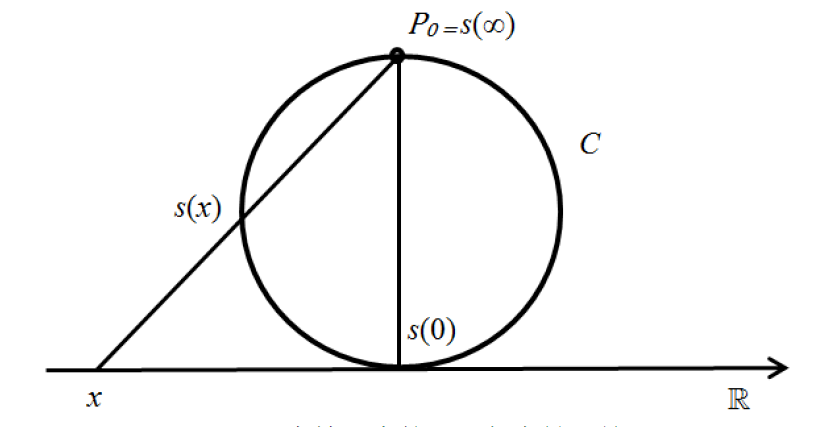
\includegraphics[scale=0.4]{去掉一点的圆周与实轴对等.png}
\caption{去掉一点的圆周与实轴对等}
\label{figure:去掉一点的圆周与实轴对等}
\end{figure}
\end{proof}

\begin{lemma}\label{lemma:映射定义域与陪域的无交分解}
设 $A, B$ 为非空集, 若 $f : A \to B$, $g : B \to A$, 则 $A$ 与 $B$ 存在如下分解:
\begin{enumerate}[(i)]
\item $A = A_1 \cup A_2$, $B = B_1 \cup B_2$;
\item $A_1 \cap A_2 = \varnothing$, $B_1 \cap B_2 = \varnothing$;
\item $f(A_1) = B_1$, $g(B_2) = A_2$.
\end{enumerate}
\end{lemma}
\begin{proof}
作集族
\begin{align*}
\Gamma = \{E \subset A : E \cap g(B - f(E)) = \varnothing\}
\end{align*}
$\Gamma$ 中的元称为 $A$ 中的\textbf{隔离集}. 令 $A_1 = \underset{E \in \Gamma}{\cup} E$, 则 $A_1 \in \Gamma$. 实际上, 对任意的 $E \in \Gamma$, 都有 $E \subset A_1$, 再由 $E \cap g(B - f(E)) = \varnothing$ 知
\begin{align*}
E \cap g(B - f(A_1)) = \varnothing
\end{align*}
从而
\begin{align*}
A_1 \cap g(B - f(A_1)) = \underset{E \in \Gamma}{\cup}[E \cap g(B - f(E))] = \varnothing
\end{align*}
因此, $A_1$ 是 $A$ 中隔离集, 且是 $\Gamma$ 中的最大元.

现在令 $B_1 = f(A_1)$, $B_2 = B - B_1$, $A_2 = g(B_2)$, 则
\begin{align*}
A_1 \cap A_2 = A_1 \cap g(B - f(A_1)) = \varnothing
\end{align*}
下面只需验证 $A_1 \cup A_2 = A$.

若不然, 则存在 $x_0 \in A$, $x_0 \notin A_1 \cup A_2$. 令 $A_0 = A_1 \cup \{x_0\}$, 由于 $B_1 = f(A_1) \subset f(A_0)$, 故
\begin{align*}
B - f(A_0) \subset B - B_1 = B_2
\end{align*}
从而
\begin{align*}
g(B - f(A_0)) \subset g(B_2) = A_2
\end{align*}
再由 $A_1 \cap A_2 = \varnothing$ 以及 $x_0 \notin A_2$ 知
\begin{align*}
A_1 \cap g(B - f(A_0)) = \varnothing, \quad x_0 \notin g(B - f(A_0))
\end{align*}
因此
\begin{align*}
A_0 \cap g(B - f(A_0)) = \varnothing
\end{align*}
故 $A_0 \in \Gamma$. 这与 $A_1$ 是 $\Gamma$ 中的最大元矛盾. 
\end{proof}

\subsection{集合的基数(势)}

\begin{definition}[集合的基数(势)]\label{definition:集合的基数(势)}
设 $A, B$ 为两个集合, 若 $A \sim B$, 则称 $A$ 与 $B$ 的\textbf{基数或势相同}, 记为 $\overline{\overline{A}} = \overline{\overline{B}}$.
\end{definition}
\begin{note}
基数反映了对等集在元素数量级别上的共性. 
\end{note}

\begin{theorem}
\begin{enumerate}[(1)]
\item 自反性:$\overline{\overline{A}} = \overline{\overline{A}}$ 。

\item 对称性:若 $\overline{\overline{A}} = \overline{\overline{B}}$,则 $\overline{\overline{B}} = \overline{\overline{A}}$ 。

\item 传递性:若 $\overline{\overline{A}} = \overline{\overline{B}}$,$\overline{\overline{B}} = \overline{\overline{C}}$,则 $\overline{\overline{A}} = \overline{\overline{C}}$ 。
\end{enumerate}
\end{theorem}
\begin{proof}
由\refthe{theorem:对等关系也是等价关系}及\hyperref[definition:集合的基数(势)]{集合的基数(势)的定义}可直接得到.
\end{proof}

\begin{definition}\label{definition:集合的基数大小关系}
对于集合 $A, B$,若有 $B_0 \subset B$,$A \sim B_0$,则称 $A$ 的基数小于等于 $B$ 的基数,记作 $\overline{\overline{A}} \leqslant\overline{\overline{B}}$。若 $\overline{\overline{A}}\leqslant \overline{\overline{B}}$ 且 $A$ 与 $B$ 不对等,则称 $A$ 的基数小于 $B$ 的基数,记作 $\overline{\overline{A}} < \overline{\overline{B}}$。
同理可定义$\overline{\overline{A}}\geqslant \overline{\overline{B}}$和$\overline{\overline{A}}> \overline{\overline{B}}$.
\end{definition}

\begin{proposition}[映射与基数之间的关系]\label{proposition:映射与基数之间的关系}
\begin{enumerate}[(1)]
\item 若存在从 $A$ 到 $B$ 的单射, 则 $\overline{\overline{A}} \leqslant \overline{\overline{B}}$;
\item 若存在从 $A$ 到 $B$ 的满射, 则 $\overline{\overline{A}} \geqslant \overline{\overline{B}}$;
\item 若存在从 $A$ 到 $B$ 的一一映射, 则 $\overline{\overline{A}} = \overline{\overline{B}}$.
\end{enumerate}
\end{proposition}
\begin{proof}
\begin{enumerate}[(1)]
\item 

\item 

\item 
\end{enumerate}
\end{proof}

\begin{theorem}[Bernstein定理]\label{theorem:Bernstein定理}
Bernstein定理的两个等价形式:
\begin{enumerate}[(1)]
\item 若 $A$ 与 $B$ 的某子集对等, $B$ 与 $A$ 的某子集对等, 则 $A \sim B$.

\item 若集合 $A, B$ 满足 $\overline{\overline{A}} \leqslant \overline{\overline{B}}$, $\overline{\overline{B}} \leqslant \overline{\overline{A}}$, 则 $\overline{\overline{A}} = \overline{\overline{B}}$. 
\end{enumerate}
\end{theorem}
\begin{proof}
\begin{enumerate}[(1)]
\item 由题设存在单射 $f : A \to B$, $g : B \to A$, 利用\reflem{lemma:映射定义域与陪域的无交分解}可得到 $A$ 与 $B$ 的分解
\begin{align*}
A = A_1 \cup A_2, \quad B = B_1 \cup B_2\\
f(A_1) = B_1, \quad g(B_2) = A_2
\end{align*}
其中, $A_1 \cap A_2 = \varnothing$, $B_1 \cap B_2 = \varnothing$. 注意到 $f : A_1 \to B_1$, $g^{-1} : A_2 \to B_2$ 是一一映射, 作映射
\begin{align*}
F(x) = 
\begin{cases}
f(x), & x \in A_1\\
g^{-1}(x), & x \in A_2
\end{cases}
\end{align*}
则 $F : A \to B$ 是一一映射, 从而 $A \sim B$.

\item 由\refdef{definition:集合的基数(势)}和\refdef{definition:集合的基数大小关系}可知(2)$\Leftrightarrow$(1).
\end{enumerate}
\end{proof}

\begin{example}\label{example:[-1,1]与R对等}
$[-1, 1] \sim \mathbb{R}$.
\end{example}
\begin{proof}
由\refexa{example-214234210.2}可知, $\mathbb{R} \sim (-1, 1) \subset [-1, 1]$; 又 $[-1, 1] \sim [-1, 1] \subset \mathbb{R}$. 由\hyperref[theorem:Bernstein定理]{Bernstein定理(1)}可知, $[-1, 1] \sim \mathbb{R}$.
\end{proof}

\begin{theorem}
对于集合 $A, B$,$\overline{\overline{A}} < \overline{\overline{B}}$,$\overline{\overline{A}} = \overline{\overline{B}}$,$\overline{\overline{A}} > \overline{\overline{B}}$ 中的任意两个不会同时成立。
\end{theorem}
\begin{proof}
由\refdef{definition:集合的基数大小关系}可知,若 $\overline{\overline{A}} = \overline{\overline{B}}$,则$A$ 与 $B$ 对等,另外两个不会成立;假设$\overline{\overline{A}} < \overline{\overline{B}}$ 与 $\overline{\overline{A}} > \overline{\overline{B}}$ 同时成立,则存在$B_0 \subset B$,$A_0 \subset A$,使得$A \sim B_0$,$B \sim A_0$.使用\hyperref[theorem:Bernstein定理]{Bernstein定理(1)}得出$A \subset B$,进而$\overline{\overline{A}} = \overline{\overline{B}}$,显然矛盾,证毕。
\end{proof}

\begin{definition}[有限集与无限集]\label{definition:有限集与无限集}
设$A$是一个非空集合,若存在自然数 $n$, 使得 $A \sim \{1, 2, \cdots, n\}$, 则称 $A$ 为\textbf{有限集}, 并记 $\overline{\overline{A}} = n$. 若$A$不是有限集,则称$A$为\textbf{无限集}.特别地,规定 $\overline{\overline{\varnothing}} = 0$.
\end{definition}
\begin{note}
由上述定义可知有限集的基数等于该集合元素的个数. 实际上, 集合的基数就是有限集元素个数的推广.
\end{note}

\begin{theorem}
设$A$是非空集合,则
\begin{enumerate}[(1)]
\item $A$是有限集的充要条件是$A$不与其任何真子集对等.
\item $A$是无限集的充要条件是$A$与其某个真子集对等.
\end{enumerate}
\end{theorem}
\begin{note}
这就是有限集与无限集的本质区别.
\end{note}
\begin{proof}
先证(1)(2)的必要性.

(1)的必要性:设$\overline{\overline{A}} = n$,用数学归纳法证明, $n = 1$, 显然. 假设 $n = k$ 时, 结论成立.

当 $n = k + 1$ 时, 若存在 $A$ 的某个真子集 $A_0$ 使得 $A \sim A_0$, 则存在一一映射 $\varphi : A \to A_0$. 下面分两种情况:

(i) $\exists a \in A$, 使得 $\varphi(a) = a$.

令 $A_1 = A - \{a\}$, $A_2 = A_0 - \{a\}$, 则 $A_2$ 是 $A_1$ 的真子集, $\overline{\overline{A_1}} = k$. 而 $\varphi|_{A_1}$ 是 $A_1$ 到 $A_2$ 的一一映射, 故 $A_1 \sim A_2$. 这与假设矛盾.

(ii) $\forall a \in A$, 都有 $\varphi(a) \neq a$.

$A_0$ 是 $A$ 的真子集, 则存在 $x_0 \in A$, $x_0 \notin A_0$. 令
\begin{align*}
A_3 = A - \{x_0\}, \quad A_4 = A_0 - \{\varphi(x_0)\}
\end{align*}
注意到 $x_0 \notin A_0$ 以及 $A_0$ 是 $A$ 的真子集, 则 $A_4$ 是 $A_3$ 的子集. 又由于
\begin{align*}
\varphi(x_0) \in A_0 \subset A, \quad \varphi(x_0) \neq x_0
\end{align*}
故 $\varphi(x_0) \in A - \{x_0\} = A_3$, 而 $\varphi(x_0) \notin A_0 - \{\varphi(x_0)\} = A_4$. 从而 $A_4$ 是 $A_3$ 的真子集, 于是 $\overline{\overline{A_3}} = k$, $\varphi|_{A_3}$ 是 $A_3$ 到 $A_4$ 的一一映射, 故 $A_3 \sim A_4$. 这与假设矛盾. 

(2)的必要性:设$A$是无限集.先证明在任一无限集 $A$ 中, 一定能取出一列互不相同的元素 $a_1, a_2, \cdots$. 事实上, 在 $A$ 中任取一个元素, 记为 $a_1$. 因为 $A$ 是无限集, 集 $A - \{a_1\}$ 显然不空, 这时再从集 $A - \{a_1\}$ 取一个元素 $a_2$, 同样, $A - \{a_1, a_2\}$ 决不空. 可以继续做下去, 将从 $A$ 中取出一列互不相同的元素 $a_1, a_2, \cdots$, 记余集为 $\hat{A} = A - \{a_n | n = 1, 2, \cdots\}$. 在 $A$ 中取出一个真子集
\begin{align*}
\{a_2, a_3, \cdots\} \cup \hat{A} = \tilde{A}
\end{align*}
现作 $A$ 与 $\tilde{A}$ 之间的映射 $\varphi$:
\begin{align*}
&\varphi(a_i) = a_{i + 1}, \quad i = 1, 2, \cdots\\
&\varphi(x) = x, \quad x \in \hat{A}
\end{align*}
显然, $\varphi$ 是 $A$ 到 $\tilde{A}$ 上的一一对应, 证毕. 

再证(1)(2)的充分性.

(1)的充分性:设$A$不与其任何真子集对等,假设$A$是无限集,则与由(2)的必要性矛盾!因此$A$不是无限集,故$A$是有限集.

(2)的充分性:设$A$与其某个真子集对等,假设$A$是有限集,则与(1)的必要性矛盾!因此$A$是不是有限集.故$A$一定是无限集.
\end{proof}









\end{document}